\subsection{Согласованная фильтрация линейно-частотно
модулированного сигнала}
В этом задании на примере ЛЧМ сигнала подробно исследуются
особенности фильтрации сложных сигналов. 

%Выбрать среднюю частоту заполнения 1000Гц,
%длительность ЛЧМ сигнала менять в пределах от 10мс до 100мс
%девиацию частоты изменять от 400Гц до 1000Гц 

%Пропустить ЛАМ сигнал через согласованный фильтр. Качественно
%проанализировать, чем определяются основные параметры выходного сигнала:
%величина его максимума и степень укорочения сигнала, временное положение
%максимума. Получить и построить графики следующих зависимостей, оставляя
%среднюю частоту неизменной:


\subsubsection{Исследование зависимостей длительности выходного сигнала }%



\paragraph{Зависимость длительности выходного сигнала от длительности входного сигнала}%
\begin{figure}[H]
    \centering
    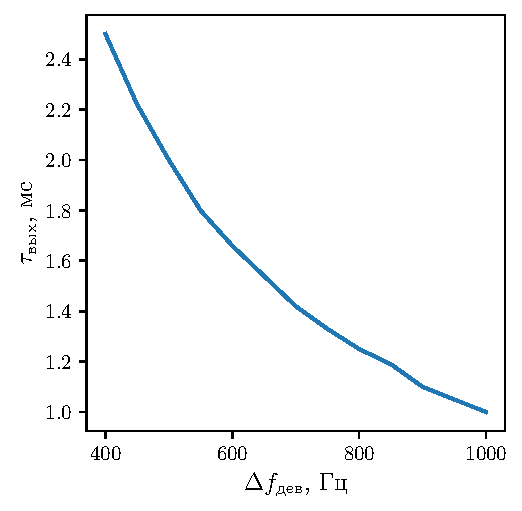
\includegraphics[width=0.6\linewidth]{imgs/task3/t3f0}
    \caption{}
    \label{fig:3.1}
\end{figure}
Зависит прямо пропорциональна, так как пиковое значение выходного сигнала
согласованного фильтра достигается не раньше, чем окончится импульсный сигнал,
поступающий на вход фильтра. Иначе невозможно накопить всю энергию входного
сигнала для формирования пика на выходе фильтра в момент времени $t_0$.
Увеличение $t_0$ сверх величины $\tau + T$ не влияет на величину максимума
выходного сигнала, а лишь сдвигает его в сторону большего запаздывания. Поэтому
имеет смысл выбирать $t_0 = \tau + T$. Тогда максимальное значение выходного
сигнала достигается точно в момент окончания входного импульса. В данном
эксперименте пиковое значение достигается в момент времени окончания входного
сигнала, так как сигнал $M(t)$ достигает максимального значения в момент $t_0$,
поскольку функция корреляции всегда имеет максимальное значение в нуле 
\begin{equation}
    \Psi^{max}_m(\tau) = \Psi_m(0)
\end{equation}
Тогда максимальное значение с точностью до постоянного множителя $C_0$
равно энергии сигнала: Формула (35)

\paragraph{Зависимость длительности выходного сигнала от девиации частоты входного сигнала}%
При увеличении девиации входного сигнала уменьшается длительность выходного
сигнала см. рис. \ref{fig:3.1}

Сжатие сигнала (его укорочение) прямо пропорционально базе сигнала. В случае
ЛЧМ сигнала база сигнала регулируется значением девиации частоты.  При
увеличении девиации уменьшается $\tau$ - характерное время выходного сигнала (см
формулу 53). При уменьшении $\tau$ увеличивается характерная ширина спектра
выходного сигнала (как следствие из Фурье-преобразования). Получаем, что при
увеличении девиации сигнала увеличивается его база.



\paragraph{Зависимость амплитуды выходного сигнала от длительности входного сигнала}%

Прямо пропорциональна (см. рис. \ref{fig:3.2}) так как при увеличении длительности
входного сигнала увеличивается суммарная энергия сигнала, и, как следствие,
увеличивается амплитуда выходного сигнала.

\begin{figure}[H]
    \centering
    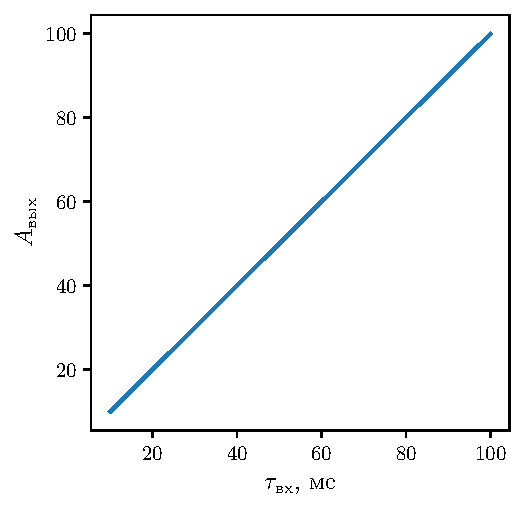
\includegraphics[width=0.6\linewidth]{imgs/task3/t3f1}
    \caption{}
    \label{fig:3.2}
\end{figure}

\paragraph{Зависимость амплитуды максимума выходного сигнала от девиации частоты входного сигнала}%
Зависимости нет, девиация частоты максимума входного сигнала не влияет на
амплитуду выходного.  Однако для других значений есть зависимость — так как при
изменении девиации входного сигнала изменяется длительность выходного сигнала
(при увеличении девиации длительность уменьшается), а значит при увеличении
девиации в любых значениях кроме максимального значения амплитуды амплитуда
выходного сигнала будет уменьшаться (при рассмотрении участка до первого нуля —
дальше значения амплитуды будут колебаться). 


\paragraph{Зависимость временного положения максимума от длительности входного сигнала}%


\begin{figure}[H]
    \centering
    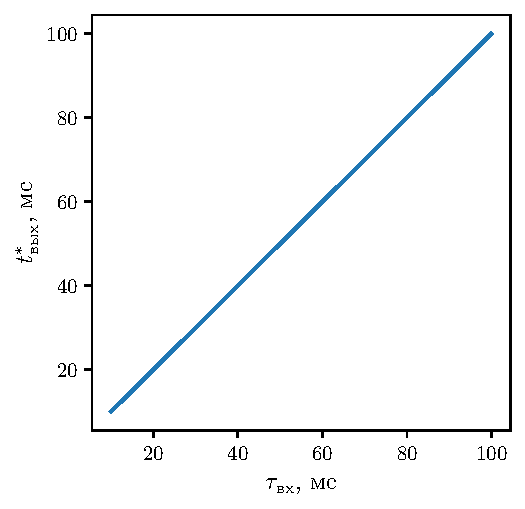
\includegraphics[width=0.6\linewidth]{imgs/task3/t3f2}
    \caption{}
    \label{fig:3.3}
\end{figure}

Прямо пропорциональна длительности входного сигнала (см. рис. \ref{fig:3.3}). Положение максимума
выходного сигнала для ЛЧМ сигнала равно времени окончания входного сигнала.

\paragraph{Зависимость временного положения максимума от девиации частоты входного сигнала}%

Не зависит. Девиация частоты не оказывает влияния на значение максимума выходного сигнала (как на его временное положение, так и на его амлитуду)

